\documentclass{standalone}
\usepackage{tikz}
\usetikzlibrary{patterns, positioning}


\begin{document}
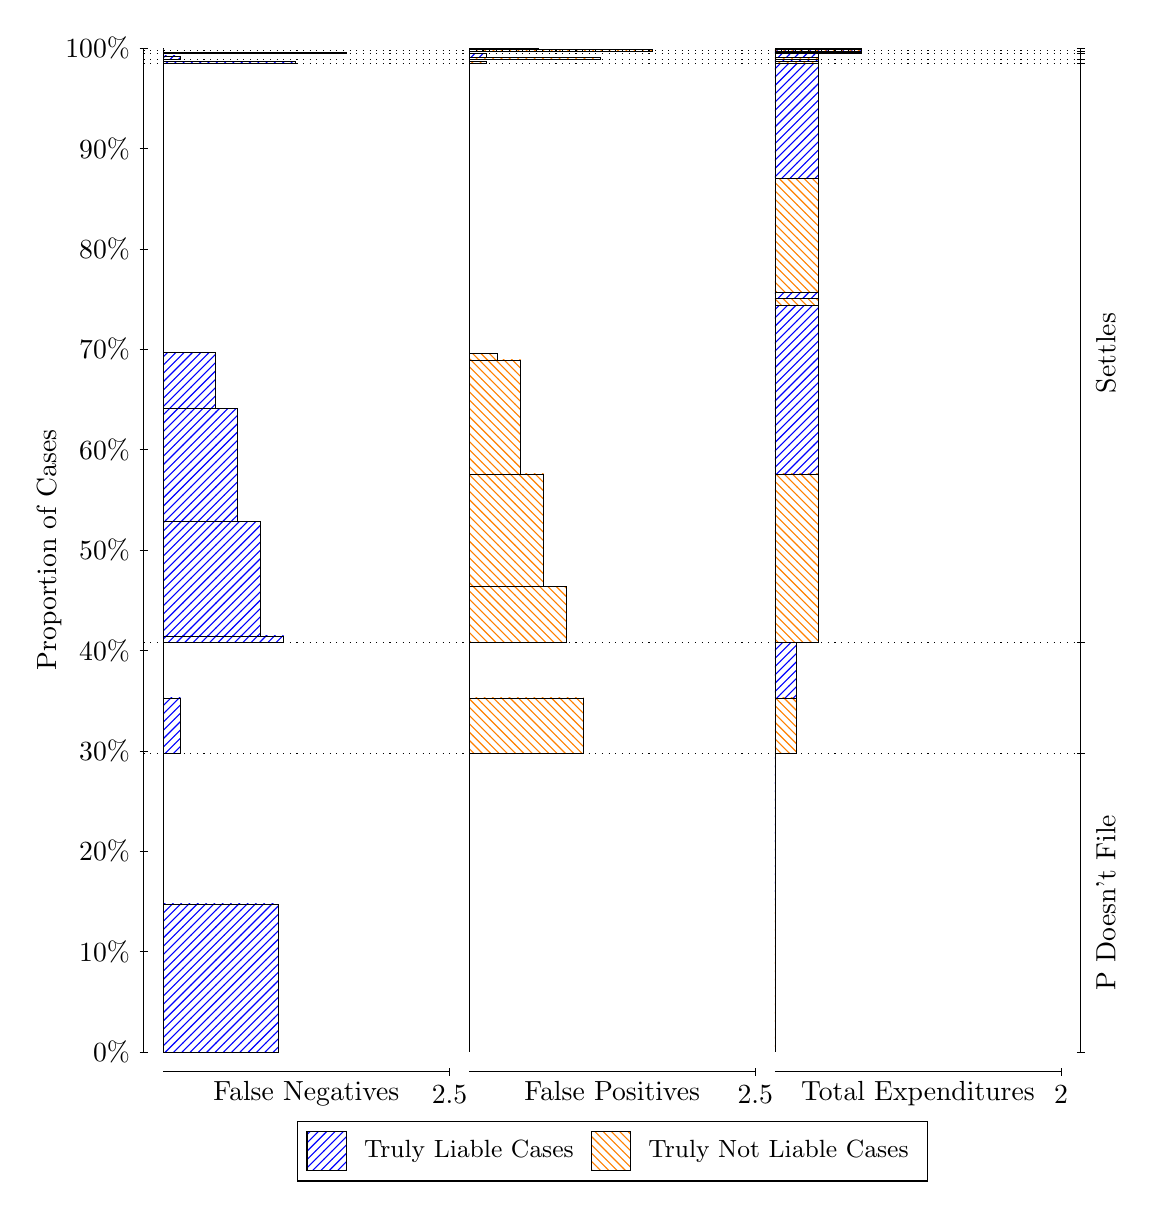
\begin{tikzpicture}
\draw[black, very thin] (1.5,1.75) -- (1.5,14.5);
\node[rotate=90, text=black, anchor=center] at (0.3, 8.125) {Proportion of Cases};
\draw[black, very thin] (1.45,1.75) -- (1.55,1.75);
\node[text=black, anchor=east] at (1.45, 1.75) {0\%};
\draw[black, very thin] (1.45,3.025) -- (1.55,3.025);
\node[text=black, anchor=east] at (1.45, 3.025) {10\%};
\draw[black, very thin] (1.45,4.3) -- (1.55,4.3);
\node[text=black, anchor=east] at (1.45, 4.3) {20\%};
\draw[black, very thin] (1.45,5.575) -- (1.55,5.575);
\node[text=black, anchor=east] at (1.45, 5.575) {30\%};
\draw[black, very thin] (1.45,6.85) -- (1.55,6.85);
\node[text=black, anchor=east] at (1.45, 6.85) {40\%};
\draw[black, very thin] (1.45,8.125) -- (1.55,8.125);
\node[text=black, anchor=east] at (1.45, 8.125) {50\%};
\draw[black, very thin] (1.45,9.4) -- (1.55,9.4);
\node[text=black, anchor=east] at (1.45, 9.4) {60\%};
\draw[black, very thin] (1.45,10.675) -- (1.55,10.675);
\node[text=black, anchor=east] at (1.45, 10.675) {70\%};
\draw[black, very thin] (1.45,11.95) -- (1.55,11.95);
\node[text=black, anchor=east] at (1.45, 11.95) {80\%};
\draw[black, very thin] (1.45,13.225) -- (1.55,13.225);
\node[text=black, anchor=east] at (1.45, 13.225) {90\%};
\draw[black, very thin] (1.45,14.5) -- (1.55,14.5);
\node[text=black, anchor=east] at (1.45, 14.5) {100\%};

\draw[black, very thin] (13.4,1.75) -- (13.4,14.5);
\draw[black, very thin] (13.35,1.75) -- (13.45,1.75);
\node[anchor=west] at (13.35, 1.75) {};
\draw[black, very thin] (13.35,5.5385) -- (13.45,5.5385);
\node[anchor=west] at (13.35, 5.5385) {};
\draw[black, very thin] (13.35,6.9552) -- (13.45,6.9552);
\node[anchor=west] at (13.35, 6.9552) {};
\draw[black, very thin] (13.35,14.3) -- (13.45,14.3);
\node[anchor=west] at (13.35, 14.3) {};
\draw[black, very thin] (13.35,14.358) -- (13.45,14.358);
\node[anchor=west] at (13.35, 14.358) {};
\draw[black, very thin] (13.35,14.429) -- (13.45,14.429);
\node[anchor=west] at (13.35, 14.429) {};
\draw[black, very thin] (13.35,14.464) -- (13.45,14.464);
\node[anchor=west] at (13.35, 14.464) {};
\draw[black, very thin] (13.35,14.5) -- (13.45,14.5);
\node[anchor=west] at (13.35, 14.5) {};

\draw[black, very thin, pattern color=blue, pattern=north east lines] (1.75,1.75) rectangle (3.2033,3.6315);
\draw[black, very thin, pattern color=orange, pattern=north west lines] (1.75,3.6315) rectangle (1.75,5.5385);
\draw[black, very thin, pattern color=blue, pattern=north east lines] (1.75,5.5385) rectangle (1.968,6.2468);
\draw[black, very thin, pattern color=orange, pattern=north west lines] (1.75,6.2468) rectangle (1.75,6.9552);
\draw[black, very thin, pattern color=blue, pattern=north east lines] (1.75,6.9552) rectangle (3.276,7.0343);
\draw[black, very thin, pattern color=blue, pattern=north east lines] (1.75,7.0343) rectangle (2.9853,8.4891);
\draw[black, very thin, pattern color=blue, pattern=north east lines] (1.75,8.4891) rectangle (2.6947,9.9221);
\draw[black, very thin, pattern color=blue, pattern=north east lines] (1.75,9.9221) rectangle (2.404,10.63);
\draw[black, very thin, pattern color=orange, pattern=north west lines] (1.75,10.63) rectangle (1.75,14.3);
\draw[black, very thin, pattern color=blue, pattern=north east lines] (1.75,14.3) rectangle (3.4213,14.329);
\draw[black, very thin, pattern color=orange, pattern=north west lines] (1.75,14.329) rectangle (1.75,14.358);
\draw[black, very thin, pattern color=blue, pattern=north east lines] (1.75,14.358) rectangle (1.968,14.401);
\draw[black, very thin, pattern color=orange, pattern=north west lines] (1.75,14.401) rectangle (1.75,14.429);
\draw[black, very thin, pattern color=blue, pattern=north east lines] (1.75,14.429) rectangle (4.0753,14.446);
\draw[black, very thin, pattern color=orange, pattern=north west lines] (1.75,14.446) rectangle (1.75,14.464);
\draw[black, very thin, pattern color=orange, pattern=north west lines] (1.75,14.464) rectangle (1.75,14.48);
\draw[black, very thin, pattern color=blue, pattern=north east lines] (1.75,14.48) rectangle (1.75,14.5);
\draw[black, very thin, pattern color=orange, pattern=north west lines] (5.6333,1.75) rectangle (5.6333,3.657);
\draw[black, very thin, pattern color=blue, pattern=north east lines] (5.6333,3.657) rectangle (5.6333,5.5385);
\draw[black, very thin, pattern color=orange, pattern=north west lines] (5.6333,5.5385) rectangle (7.0867,6.2468);
\draw[black, very thin, pattern color=blue, pattern=north east lines] (5.6333,6.2468) rectangle (5.6333,6.9552);
\draw[black, very thin, pattern color=orange, pattern=north west lines] (5.6333,6.9552) rectangle (6.8687,7.6635);
\draw[black, very thin, pattern color=orange, pattern=north west lines] (5.6333,7.6635) rectangle (6.578,9.0917);
\draw[black, very thin, pattern color=orange, pattern=north west lines] (5.6333,9.0917) rectangle (6.2873,10.539);
\draw[black, very thin, pattern color=orange, pattern=north west lines] (5.6333,10.539) rectangle (5.9967,10.624);
\draw[black, very thin, pattern color=blue, pattern=north east lines] (5.6333,10.624) rectangle (5.6333,14.3);
\draw[black, very thin, pattern color=orange, pattern=north west lines] (5.6333,14.3) rectangle (5.8513,14.328);
\draw[black, very thin, pattern color=blue, pattern=north east lines] (5.6333,14.328) rectangle (5.6333,14.358);
\draw[black, very thin, pattern color=orange, pattern=north west lines] (5.6333,14.358) rectangle (7.3047,14.386);
\draw[black, very thin, pattern color=blue, pattern=north east lines] (5.6333,14.386) rectangle (5.8513,14.429);
\draw[black, very thin, pattern color=orange, pattern=north west lines] (5.6333,14.429) rectangle (5.6333,14.447);
\draw[black, very thin, pattern color=blue, pattern=north east lines] (5.6333,14.447) rectangle (5.6333,14.464);
\draw[black, very thin, pattern color=orange, pattern=north west lines] (5.6333,14.464) rectangle (7.9587,14.48);
\draw[black, very thin, pattern color=blue, pattern=north east lines] (5.6333,14.48) rectangle (6.5053,14.5);
\draw[black, very thin, pattern color=orange, pattern=north west lines] (9.5167,1.75) rectangle (9.5167,3.657);
\draw[black, very thin, pattern color=blue, pattern=north east lines] (9.5167,3.657) rectangle (9.5167,5.5385);
\draw[black, very thin, pattern color=orange, pattern=north west lines] (9.5167,5.5385) rectangle (9.7892,6.2468);
\draw[black, very thin, pattern color=blue, pattern=north east lines] (9.5167,6.2468) rectangle (9.7892,6.9552);
\draw[black, very thin, pattern color=orange, pattern=north west lines] (9.5167,6.9552) rectangle (10.062,9.0917);
\draw[black, very thin, pattern color=blue, pattern=north east lines] (9.5167,9.0917) rectangle (10.062,11.233);
\draw[black, very thin, pattern color=orange, pattern=north west lines] (9.5167,11.233) rectangle (10.062,11.319);
\draw[black, very thin, pattern color=blue, pattern=north east lines] (9.5167,11.319) rectangle (10.062,11.398);
\draw[black, very thin, pattern color=orange, pattern=north west lines] (9.5167,11.398) rectangle (10.062,12.845);
\draw[black, very thin, pattern color=blue, pattern=north east lines] (9.5167,12.845) rectangle (10.062,14.3);
\draw[black, very thin, pattern color=orange, pattern=north west lines] (9.5167,14.3) rectangle (10.062,14.328);
\draw[black, very thin, pattern color=blue, pattern=north east lines] (9.5167,14.328) rectangle (10.062,14.358);
\draw[black, very thin, pattern color=orange, pattern=north west lines] (9.5167,14.358) rectangle (10.062,14.386);
\draw[black, very thin, pattern color=blue, pattern=north east lines] (9.5167,14.386) rectangle (10.062,14.429);
\draw[black, very thin, pattern color=orange, pattern=north west lines] (9.5167,14.429) rectangle (10.607,14.447);
\draw[black, very thin, pattern color=blue, pattern=north east lines] (9.5167,14.447) rectangle (10.607,14.464);
\draw[black, very thin, pattern color=orange, pattern=north west lines] (9.5167,14.464) rectangle (10.607,14.48);
\draw[black, very thin, pattern color=blue, pattern=north east lines] (9.5167,14.48) rectangle (10.607,14.5);
\draw[black, dotted] (1.5,5.5385) -- (13.4,5.5385);
\draw[black, dotted] (1.5,6.9552) -- (13.4,6.9552);
\draw[black, dotted] (1.5,14.3) -- (13.4,14.3);
\draw[black, dotted] (1.5,14.358) -- (13.4,14.358);
\draw[black, dotted] (1.5,14.429) -- (13.4,14.429);
\draw[black, dotted] (1.5,14.464) -- (13.4,14.464);
\draw[black, very thin] (1.75,1.5) -- (5.3833,1.5);
\node[text=black, anchor=north] at (3.5667, 1.5) {False Negatives};
\draw[black, very thin] (5.3833,1.45) -- (5.3833,1.55);
\node[text=black, anchor=north] at (5.3833, 1.45) {2.5};

\draw[black, very thin] (5.6333,1.5) -- (9.2667,1.5);
\node[text=black, anchor=north] at (7.45, 1.5) {False Positives};
\draw[black, very thin] (9.2667,1.45) -- (9.2667,1.55);
\node[text=black, anchor=north] at (9.2667, 1.45) {2.5};

\draw[black, very thin] (9.5167,1.5) -- (13.15,1.5);
\node[text=black, anchor=north] at (11.333, 1.5) {Total Expenditures};
\draw[black, very thin] (13.15,1.45) -- (13.15,1.55);
\node[text=black, anchor=north] at (13.15, 1.45) {2};

\node[text=black, centered, rotate=90] at (13.72, 3.6442) {P Doesn't File};

\node[text=black, centered, rotate=90] at (13.72, 10.627) {Settles};





\draw (7.449999999999999,1.5) node[draw=none] (baseCoordinate) {};
\begin{scope}[align=center]
        \matrix[scale=0.5, draw=black, below=0.5cm of baseCoordinate, nodes={draw}, column sep=0.1cm]{
            \node[rectangle, draw, minimum width=0.5cm, minimum height=0.5cm, pattern color=blue, pattern=north east lines] {}; &
            \node[draw=none, font=\small, text=black] (B) {Truly Liable Cases}; &
            \node[rectangle, draw, minimum width=0.5cm, minimum height=0.5cm, pattern color=orange, pattern=north west lines] {}; &
            \node[draw=none, font=\small, text=black] (B) {Truly Not Liable Cases}; \\
            };
\end{scope}

\end{tikzpicture}
\end{document}